
\documentclass[12pt, a4paper]{article}

% ============================================================
% PACKAGES
% ============================================================
\usepackage[utf8]{inputenc}
\usepackage[vietnamese]{babel}       % Tiếng Việt
\usepackage[T5]{fontenc}
\usepackage{geometry}
\geometry{a4paper, margin=2.5cm}

\usepackage{amsmath, amssymb, amsthm}
\usepackage{graphicx}
\usepackage{subcaption}              % subfigure
\usepackage{float}                   % [H] placement
\usepackage{booktabs}                % đẹp cho bảng
\usepackage{multirow}
\usepackage{array}
\usepackage{xcolor}
\usepackage{hyperref}
\hypersetup{colorlinks=true, linkcolor=blue, citecolor=red, urlcolor=cyan}
\usepackage{listings}                % code snippet
\usepackage{caption}
\usepackage{enumitem}
\usepackage{titlesec}
\usepackage{fancyhdr}

% Header / Footer
\pagestyle{fancy}
\fancyhf{}
\rhead{CSC14005 -- Đồ Án 1}
\lhead{Part 2: Classification}
\cfoot{\thepage}

% Code snippet style
\lstset{
  language=Python,
  basicstyle=\ttfamily\small,
  keywordstyle=\color{blue},
  commentstyle=\color{gray},
  stringstyle=\color{orange},
  numbers=left,
  numberstyle=\tiny\color{gray},
  breaklines=true,
  frame=single,
  showstringspaces=false
}

% ============================================================
% DOCUMENT
% ============================================================
\begin{document}

% ============================================================
% TITLE PAGE
% ============================================================
\begin{titlepage}
  \centering
  \vspace*{1.5cm}
  {\Large \textbf{TRƯỜNG ĐẠI HỌC KHOA HỌC TỰ NHIÊN}\par}
  {\large KHOA CÔNG NGHỆ THÔNG TIN\par}
  \vspace{1cm}
  \rule{\linewidth}{0.5pt}
  \vspace{0.8cm}

  {\LARGE \textbf{BÁO CÁO ĐỒ ÁN 1}\par}
  \vspace{0.4cm}
  {\Large \textbf{CSC14005 -- Machine Learning}\par}
  \vspace{0.4cm}
  {\large \textbf{PHẦN 2: PHÂN LOẠI (CLASSIFICATION)}\par}
  \vspace{0.4cm}
  {\large \textit{Dataset: Adult Census Income}\par}

  \rule{\linewidth}{0.5pt}
  \vspace{1.5cm}

  \begin{tabular}{ll}
    \textbf{Nhóm:}     & Group\_01 \\[4pt]
    \textbf{Thành viên:} & Nguyễn Văn A -- 21xxxxxx \\
                         & Trần Thị B  -- 21xxxxxx \\
    \textbf{Giảng viên:} & TS. Nguyễn Văn C \\[4pt]
    \textbf{Năm học:}  & 2025 -- 2026 \\
  \end{tabular}

  \vfill
  {\large TP. Hồ Chí Minh, \today\par}
\end{titlepage}

% ============================================================
% TABLE OF CONTENTS
% ============================================================
\tableofcontents
\newpage

% ============================================================
% SECTION 1 -- GIỚI THIỆU
% ============================================================
\section{Giới thiệu}
\label{sec:intro}

Báo cáo này trình bày kết quả thực nghiệm của \textbf{Phần 2 -- Classification} trong Đồ Án 1 môn CSC14005 (Machine Learning).
Mục tiêu là xây dựng và so sánh các mô hình phân loại \emph{từ đầu} (from scratch, không dùng \texttt{sklearn} cho phần huấn luyện) nhằm phân loại thu nhập của người theo hai lớp: $\leq$50K và $>$50K.

\subsection{Bài toán}
\begin{itemize}
  \item \textbf{Dữ liệu:} Adult Census Income Dataset (UCI Repository), được lưu tại \texttt{data/adult.csv}.
  \item \textbf{Mục tiêu:} Dự đoán nhãn nhị phân \texttt{income} $\in \{0, 1\}$ ($0 \leftrightarrow {\leq}50K$, $1 \leftrightarrow {>}50K$).
  \item \textbf{Input:} 14 đặc trưng gồm tuổi, trình độ học vấn, nghề nghiệp, số giờ làm việc, \ldots
\end{itemize}

\subsection{Các mô hình đã triển khai}
Dự án triển khai 13 mô hình phân loại:
\begin{enumerate}
  \item Logistic Regression -- Gradient Descent (GD)
  \item Logistic Regression -- Newton-Raphson / IRLS
  \item Softmax Regression (Multi-class)
  \item One-vs-Rest (OvR)
  \item One-vs-One (OvO)
  \item Linear Discriminant Analysis (LDA)
  \item Quadratic Discriminant Analysis (QDA)
  \item Perceptron
  \item Regularized Logistic Regression (L1 / L2)
  \item Probit Regression
  \item Logistic Regression + Laplace Approximation
  \item Kernel Logistic Regression (RBF)
  \item Gaussian Naive Bayes
\end{enumerate}

% ============================================================
% SECTION 2 -- PHÂN TÍCH DỮ LIỆU
% ============================================================
\section{Phân tích dữ liệu (EDA)}
\label{sec:eda}

\subsection{Tổng quan bộ dữ liệu}

\begin{table}[H]
  \centering
  \caption{Thống kê tổng quan -- Adult Census Income Dataset}
  \label{tab:dataset_overview}
  \begin{tabular}{lccc}
    \toprule
    \textbf{Thuộc tính} & \textbf{Training Set} & \textbf{Test Set} & \textbf{Tổng} \\
    \midrule
    Số mẫu         & X & X & X \\
    Số đặc trưng   & 14 & 14 & 14 \\
    Lớp $\leq$50K (\%) & X\% & X\% & X\% \\
    Lớp $>$50K (\%) & X\% & X\% & X\% \\
    Missing values & X & X & X \\
    \bottomrule
  \end{tabular}
\end{table}

\subsection{Phân phối nhãn và tính imbalanced}

Bộ dữ liệu có tỷ lệ mất cân bằng lớp khoảng \textbf{3:1} (tức $\approx$75\% mẫu thuộc lớp $\leq$50K), được thể hiện ở Hình~\ref{fig:class_dist}.

\begin{figure}[H]
  \centering
  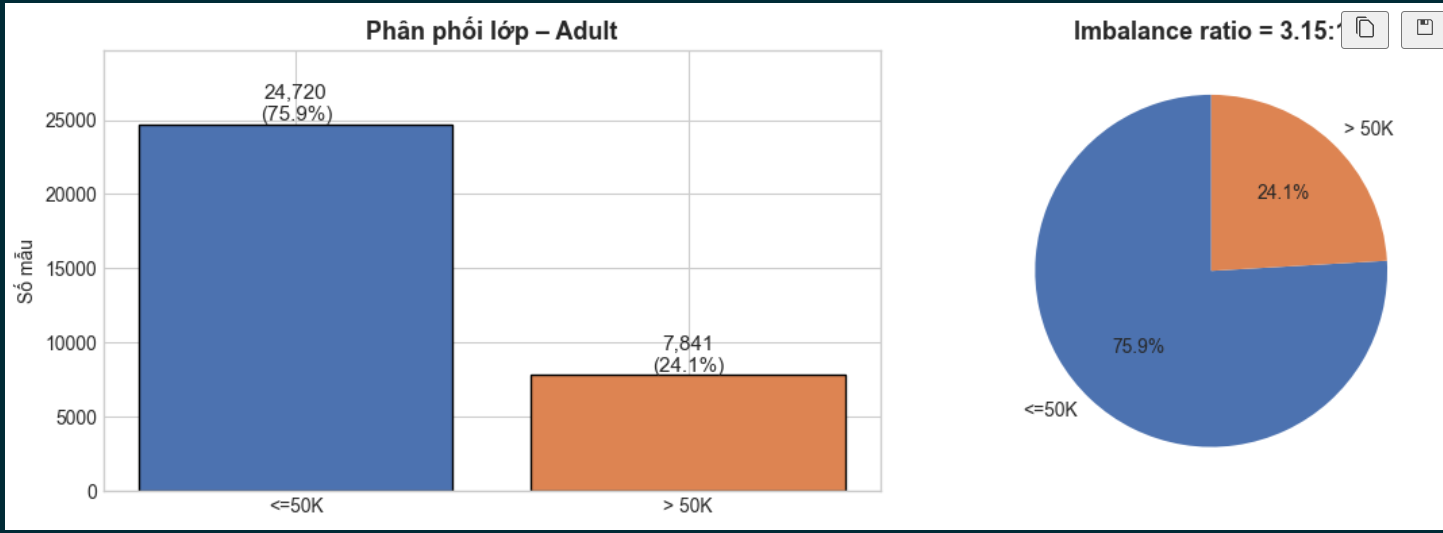
\includegraphics[width=0.75\textwidth]{figures/class_distribution.png}
  \caption{Phân phối lớp trong Adult Census Income Dataset. Imbalance ratio $\approx 3.0:1$.}
  \label{fig:class_dist}
\end{figure}

% Nhận xét ngắn về hình:
Nhận xét: Mất cân bằng lớp ($\approx$3:1) đòi hỏi phải xử lý bằng các kỹ thuật như \emph{class weighting} hoặc đánh giá bằng F1-score / AUC thay vì chỉ độ chính xác.

\subsection{Phân phối đặc trưng số theo lớp}

\begin{figure}[H]
  \centering
  \begin{subfigure}[b]{0.48\textwidth}
    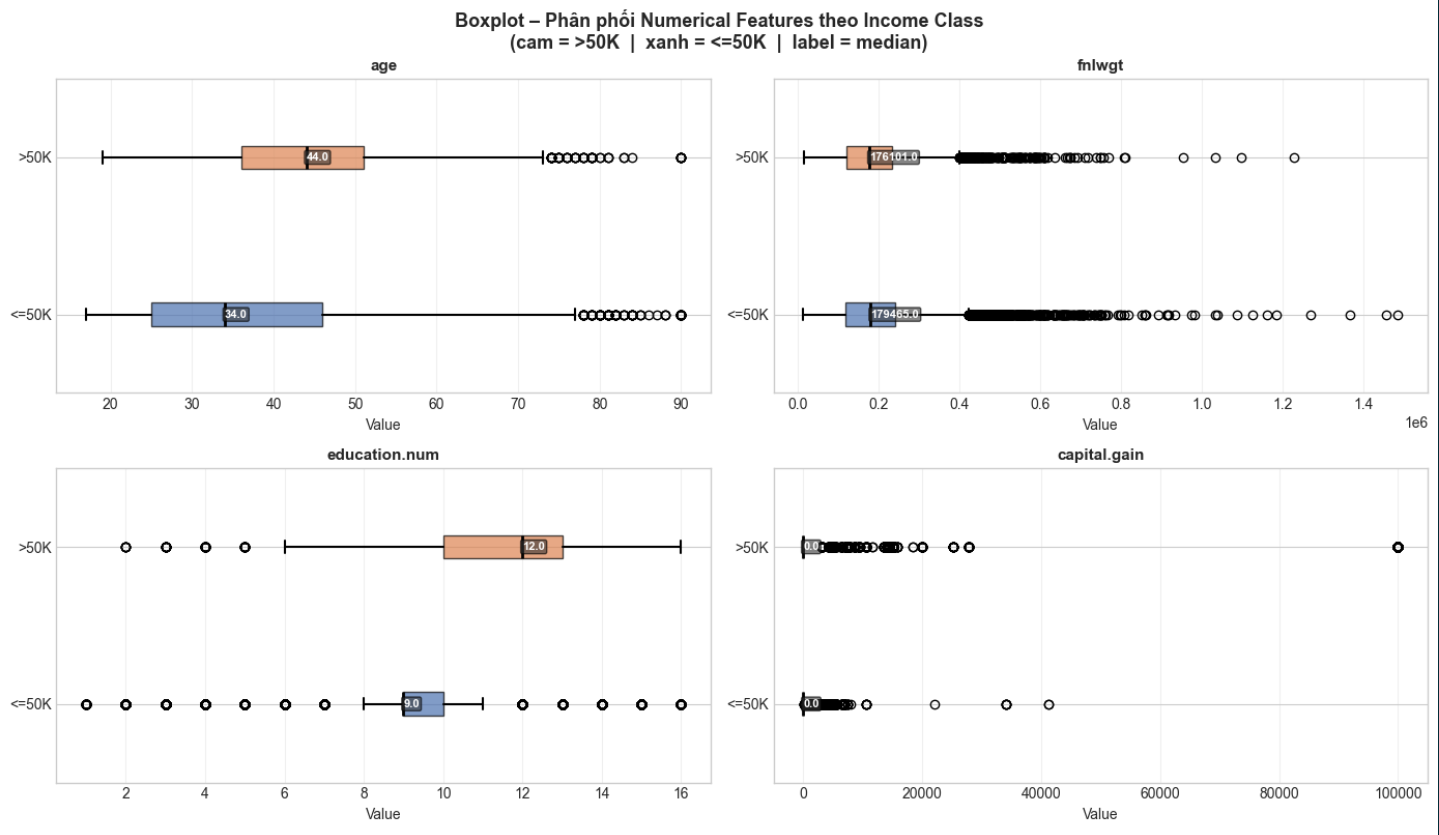
\includegraphics[width=\textwidth]{figures/boxplots_by_class.png}
    \caption{Boxplot theo lớp}
  \end{subfigure}
  \hfill
  \begin{subfigure}[b]{0.48\textwidth}
    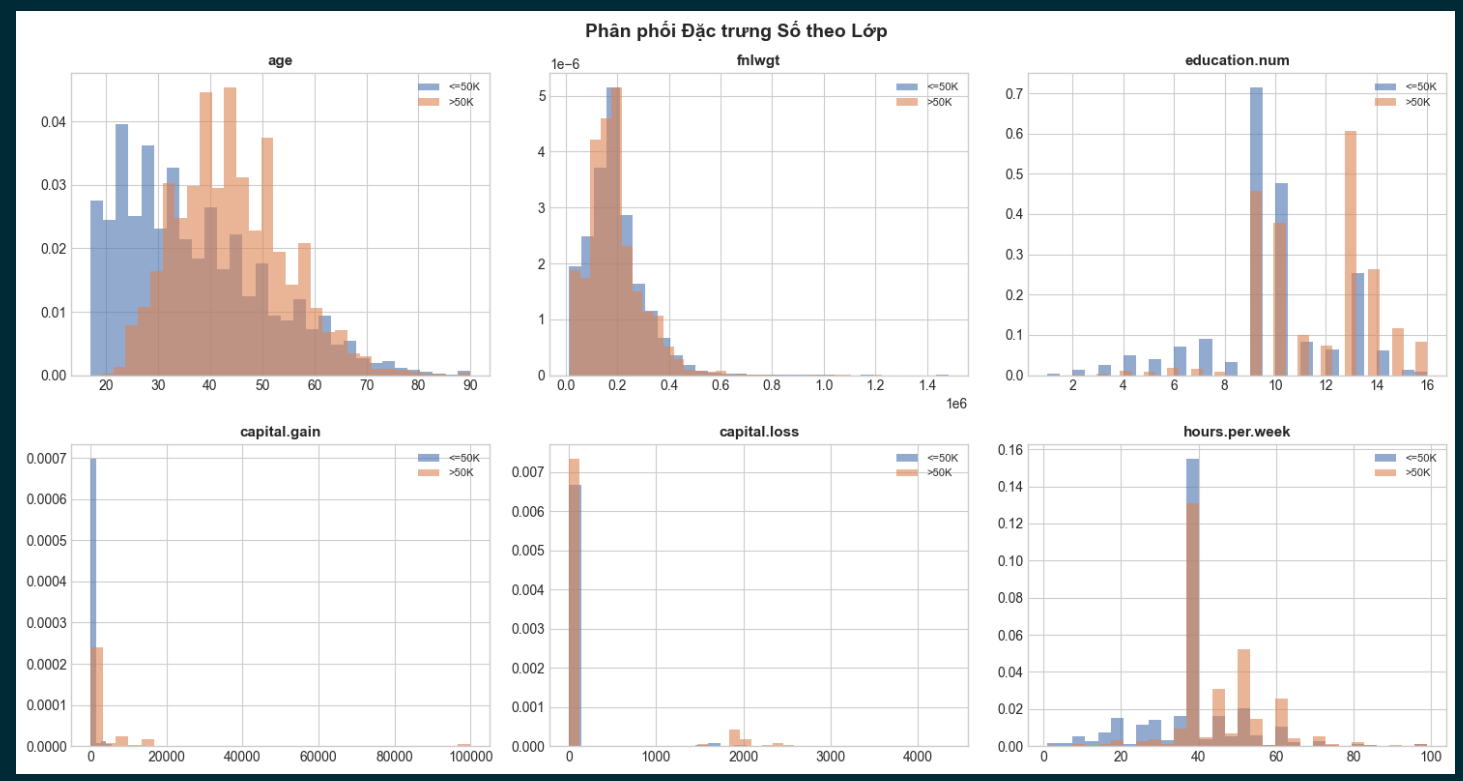
\includegraphics[width=\textwidth]{figures/histograms_by_class.png}
    \caption{Histogram theo lớp}
  \end{subfigure}
  \caption{Phân phối các đặc trưng số (\texttt{age}, \texttt{education-num}, \texttt{hours-per-week}, \ldots) theo lớp thu nhập.}
  \label{fig:feat_dist}
\end{figure}

Nhận xét:
\begin{itemize}
  \item \texttt{capital-gain} và \texttt{capital-loss}: phân phối cực kỳ lệch phải (right-skewed), đa số giá trị bằng 0.
  \item \texttt{age}: nhóm $>$50K có xu hướng nhiều tuổi hơn (median cao hơn $\approx$10 tuổi).
  \item \texttt{education-num}: nhóm thu nhập cao có trình độ giáo dục cao hơn rõ rệt.
\end{itemize}

\subsection{Phân tích ngoại lệ (Outlier Detection)}

\begin{figure}[H]
  \centering
  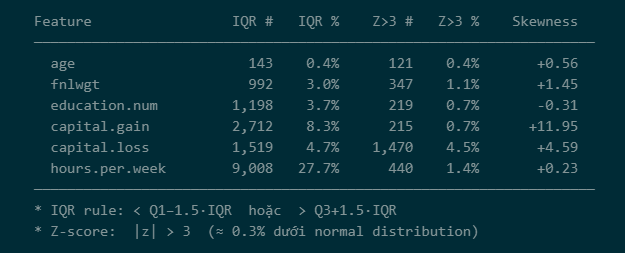
\includegraphics[width=0.85\textwidth]{figures/outlier_detection.png}
  \caption{Phân tích ngoại lệ bằng IQR và Z-score cho 3 đặc trưng có nhiều outlier nhất.}
  \label{fig:outlier}
\end{figure}

Nhận xét: \texttt{capital-gain} và \texttt{capital-loss} có tỷ lệ outlier IQR cao nhất ($\approx$X\%), chủ yếu do bản chất dữ liệu (nhiều giá trị 0 và một số giá trị rất lớn). Chúng tôi \textbf{không loại bỏ} các outlier này vì chúng mang thông tin phân loại quan trọng.

\subsection{Tương quan đặc trưng với nhãn}

\begin{figure}[H]
  \centering
  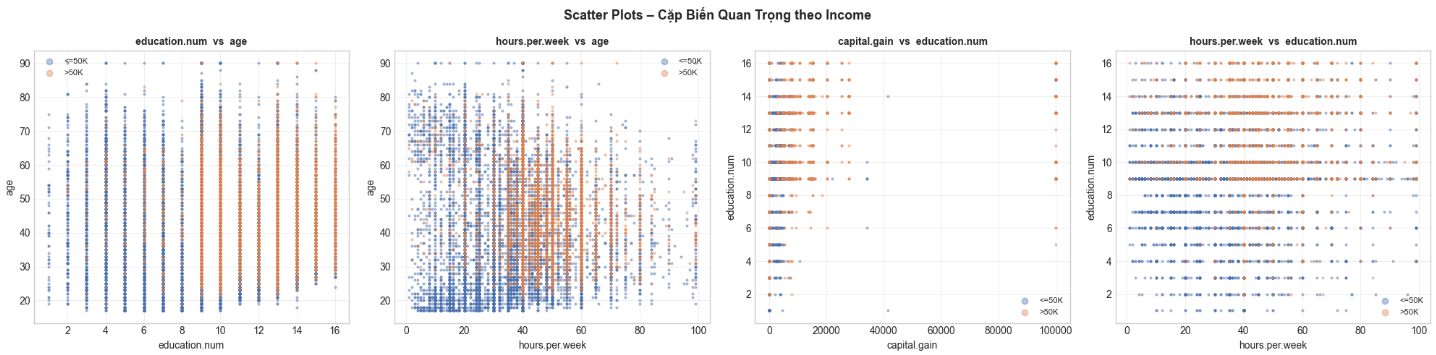
\includegraphics[width=0.70\textwidth]{figures/scatter_plots.png}
  \caption{Scatter plot các cặp đặc trưng quan trọng theo lớp thu nhập.}
  \label{fig:scatter}
\end{figure}

% ============================================================
% SECTION 3 -- TIỀN XỬ LÝ
% ============================================================
\section{Tiền xử lý dữ liệu}
\label{sec:preprocessing}

\subsection{Xử lý giá trị thiếu}
Bộ dữ liệu Adult chứa ký tự \texttt{?} thay cho giá trị thiếu trong các cột phân loại (\texttt{workclass}, \texttt{occupation}, \texttt{native-country}). Chiến lược xử lý:
\begin{itemize}
  \item Thay thế \texttt{?} bằng giá trị mode của cột tương ứng (imputation bằng most-frequent).
\end{itemize}

\subsection{Mã hóa đặc trưng phân loại}
Các đặc trưng phân loại (categorical) được mã hóa bằng \emph{Label Encoding}:
$$\text{LabelEncoder}: \texttt{workclass}, \texttt{education}, \texttt{marital-status}, \ldots \to \mathbb{Z}$$

\subsection{Chuẩn hóa đặc trưng số}
Các đặc trưng số được chuẩn hóa bằng \emph{Standardization}:
$$x' = \frac{x - \mu}{\sigma}$$
Trong đó $\mu$ và $\sigma$ được tính \textbf{chỉ trên tập train} để tránh \emph{data leakage}.

\subsection{Phân chia dữ liệu}
\begin{itemize}
  \item Train / Validation / Test: $70\%$ / $15\%$ / $15\%$ (stratified theo nhãn).
  \item Hàm: \texttt{train\_test\_split} với \texttt{random\_state=42}.
\end{itemize}

% ============================================================
% SECTION 4 -- MÔ HÌNH
% ============================================================
\section{Các mô hình phân loại}
\label{sec:models}

\subsection{Logistic Regression -- Gradient Descent}
\label{ssec:lr_gd}

\subsubsection{Nền tảng lý thuyết}

Logistic Regression mô hình hóa xác suất có điều kiện:
$$P(y=1 \mid \mathbf{x}) = \sigma(\mathbf{\theta}^\top \mathbf{x}) = \frac{1}{1 + e^{-\mathbf{\theta}^\top \mathbf{x}}}$$
trong đó $\sigma(\cdot)$ là hàm sigmoid.

\textbf{Hàm mất mát (Binary Cross-Entropy):}
$$\mathcal{L}(\mathbf{\theta}) = -\frac{1}{m}\sum_{i=1}^{m} \left[y^{(i)}\log \hat{y}^{(i)} + (1-y^{(i)})\log(1-\hat{y}^{(i)})\right]$$

\textbf{Cập nhật tham số (Gradient Descent):}
$$\mathbf{\theta} \leftarrow \mathbf{\theta} - \alpha \nabla_\theta \mathcal{L}(\mathbf{\theta})$$
với gradient:
$$\nabla_\theta \mathcal{L} = \frac{1}{m} \mathbf{X}^\top (\hat{\mathbf{y}} - \mathbf{y})$$

\textbf{Regularization:}
\begin{align*}
  \text{L2 (Ridge):} \quad & \mathcal{L}_{L2} = \mathcal{L} + \frac{\lambda}{2m}\|\mathbf{\theta}_{1:}\|^2 \\
  \text{L1 (Lasso):} \quad & \mathcal{L}_{L1} = \mathcal{L} + \frac{\lambda}{m}\|\mathbf{\theta}_{1:}\|_1
\end{align*}

\subsubsection{Siêu tham số}
\begin{table}[H]
  \centering
  \caption{Siêu tham số Logistic Regression -- GD}
  \begin{tabular}{ll}
    \toprule
    \textbf{Tham số} & \textbf{Giá trị} \\
    \midrule
    Learning rate ($\alpha$) & 0.01 \\
    Số iterations & 1000 \\
    Regularization $\lambda$ & 0.0 (mặc định) \\
    \bottomrule
  \end{tabular}
\end{table}

\subsubsection{Kết quả}

\begin{figure}[H]
  \centering
  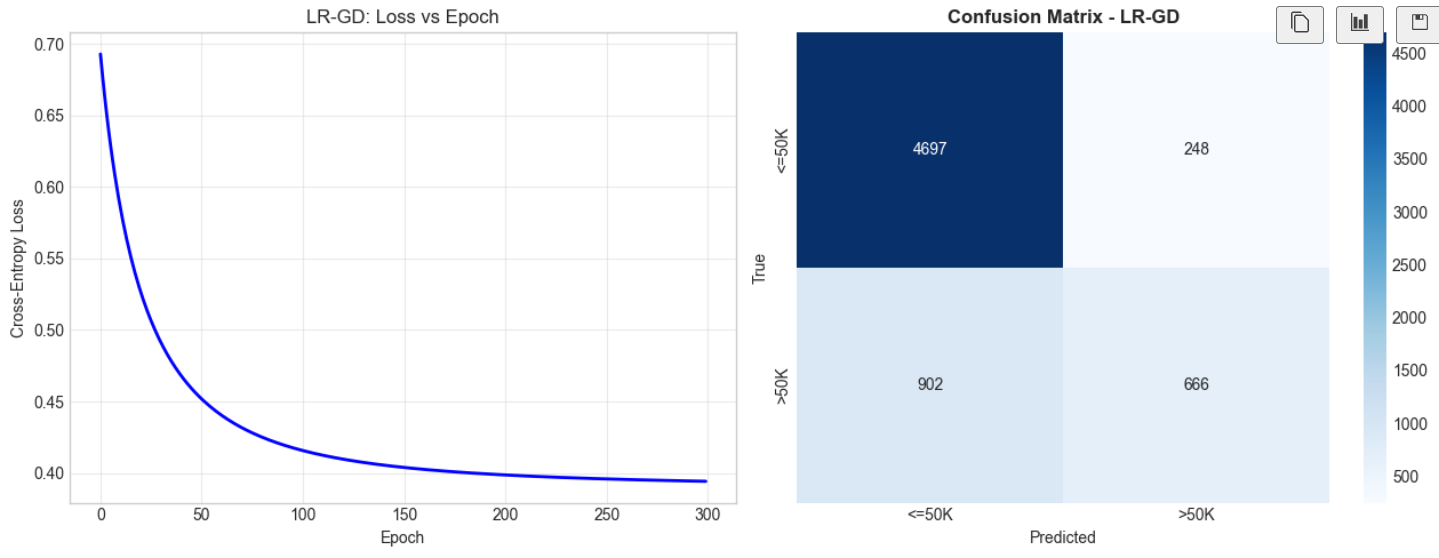
\includegraphics[width=0.75\textwidth]{figures/lr_gd_loss_cm.png}
  \caption{Loss curve và Confusion Matrix -- Logistic Regression GD.}
  \label{fig:lr_gd}
\end{figure}

% -----------------------------------------------------------

\subsection{Logistic Regression -- Newton-Raphson / IRLS}
\label{ssec:lr_newton}

\subsubsection{Nền tảng lý thuyết}

Newton-Raphson sử dụng Hessian để hội tụ nhanh hơn GD:
$$\mathbf{\theta} \leftarrow \mathbf{\theta} - \mathbf{H}^{-1} \nabla_\theta \mathcal{L}$$

\textbf{Hessian:}
$$\mathbf{H} = \frac{1}{m}\mathbf{X}^\top \mathbf{R} \mathbf{X}$$
với $\mathbf{R} = \text{diag}(\hat{y}^{(i)}(1-\hat{y}^{(i)}))$.

\subsubsection{So sánh GD vs Newton-Raphson}

\begin{figure}[H]
  \centering
  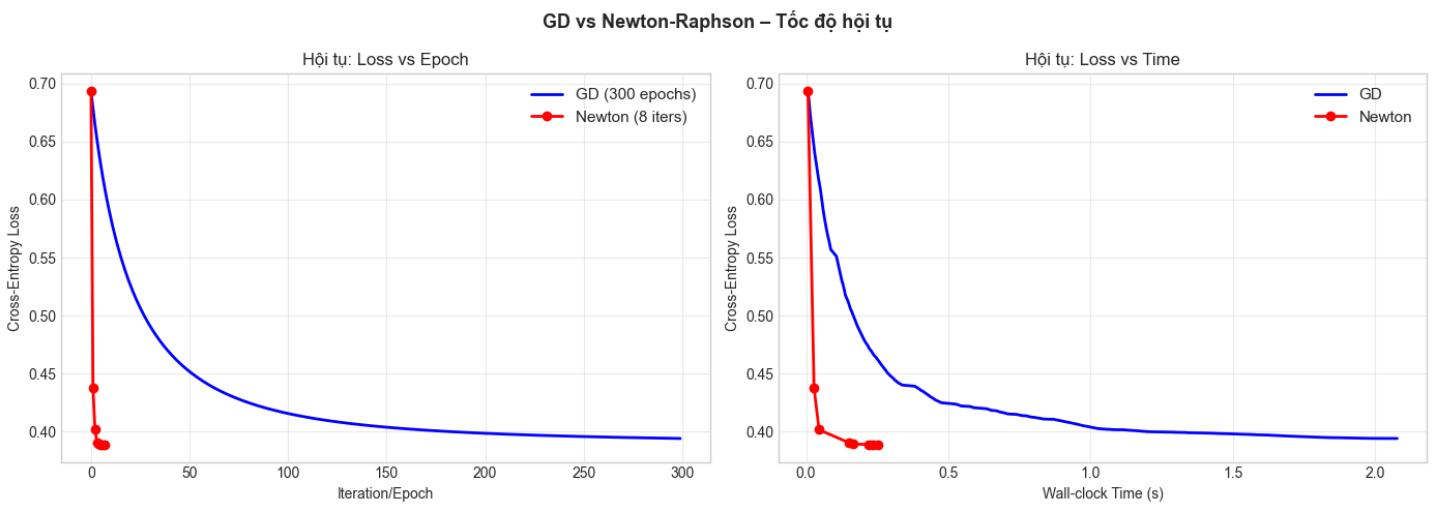
\includegraphics[width=0.75\textwidth]{figures/gd_vs_newton.png}
  \caption{Hội tụ Loss theo epochs và wall-clock time: GD vs Newton-Raphson.}
  \label{fig:gd_newton}
\end{figure}

Nhận xét: Newton-Raphson hội tụ chỉ sau $\sim$X iterations so với X iterations của GD, nhưng mỗi iteration tốn chi phí $O(nd^2)$ để tính Hessian.

% -----------------------------------------------------------

\subsection{Linear Discriminant Analysis (LDA)}
\label{ssec:lda}

\subsubsection{Nền tảng lý thuyết}

LDA là mô hình \emph{generative} giả định mỗi lớp có phân phối Gaussian với \textbf{ma trận hiệp phương sai chung}:
$$p(\mathbf{x} \mid y=k) = \mathcal{N}(\mathbf{x}; \boldsymbol{\mu}_k, \boldsymbol{\Sigma})$$

\textbf{Hàm phân biệt tuyến tính:}
$$\delta_k(\mathbf{x}) = \mathbf{x}^\top \boldsymbol{\Sigma}^{-1} \boldsymbol{\mu}_k - \frac{1}{2}\boldsymbol{\mu}_k^\top \boldsymbol{\Sigma}^{-1} \boldsymbol{\mu}_k + \log\pi_k$$

\textbf{Shared covariance:}
$$\boldsymbol{\Sigma} = \frac{1}{n - K}\sum_{k=1}^{K}\sum_{i: y_i=k} (\mathbf{x}_i - \boldsymbol{\mu}_k)(\mathbf{x}_i - \boldsymbol{\mu}_k)^\top$$

\textbf{Fisher Discriminant Ratio} đo mức độ phân biệt của từng đặc trưng:
$$\text{FDR}_j = \frac{S_B^{(j)}}{S_W^{(j)}}$$

% -----------------------------------------------------------

\subsection{Quadratic Discriminant Analysis (QDA)}
\label{ssec:qda}

QDA cho phép mỗi lớp có ma trận hiệp phương sai \textbf{riêng}:
$$p(\mathbf{x} \mid y=k) = \mathcal{N}(\mathbf{x}; \boldsymbol{\mu}_k, \boldsymbol{\Sigma}_k)$$

\textbf{Hàm phân biệt bậc hai:}
$$\delta_k(\mathbf{x}) = -\frac{1}{2}\log|\boldsymbol{\Sigma}_k| - \frac{1}{2}(\mathbf{x}-\boldsymbol{\mu}_k)^\top \boldsymbol{\Sigma}_k^{-1}(\mathbf{x}-\boldsymbol{\mu}_k) + \log\pi_k$$

\begin{table}[H]
  \centering
  \caption{So sánh số tham số: LDA vs QDA ($K=2$, $d=$ số đặc trưng)}
  \begin{tabular}{lcc}
    \toprule
    & \textbf{LDA} & \textbf{QDA} \\
    \midrule
    Mean vectors & $K \cdot d$ & $K \cdot d$ \\
    Covariance matrices & $\frac{d(d+1)}{2}$ (shared) & $K \cdot \frac{d(d+1)}{2}$ (per-class) \\
    Priors & $K-1$ & $K-1$ \\
    \midrule
    \textbf{Tổng} & $\sim Kd + d^2/2$ & $\sim Kd + Kd^2/2$ \\
    \bottomrule
  \end{tabular}
\end{table}

% -----------------------------------------------------------

\subsection{Gaussian Naive Bayes}
\label{ssec:gnb}

Naive Bayes giả định các đặc trưng \textbf{độc lập có điều kiện} (diagonal covariance):
$$p(\mathbf{x} \mid y=k) = \prod_{j=1}^{d} \mathcal{N}(x_j; \mu_{kj}, \sigma_{kj}^2)$$

Log-likelihood:
$$\log P(y=k \mid \mathbf{x}) \propto \sum_{j=1}^{d} \left[-\frac{(x_j - \mu_{kj})^2}{2\sigma_{kj}^2} - \frac{1}{2}\log(2\pi\sigma_{kj}^2)\right] + \log\pi_k$$

% -----------------------------------------------------------

\subsection{Perceptron}
\label{ssec:perceptron}

Cập nhật Perceptron (nhãn $\in \{-1, +1\}$):
$$\mathbf{w} \leftarrow \mathbf{w} + \alpha \cdot y_i \cdot \mathbf{x}_i \quad \text{nếu } y_i \cdot (\mathbf{w}^\top \mathbf{x}_i) \leq 0$$

% -----------------------------------------------------------

\subsection{Probit Regression}
\label{ssec:probit}

Probit Regression sử dụng hàm CDF Gaussian thay cho sigmoid:
$$P(y=1 \mid \mathbf{x}) = \Phi(\mathbf{\theta}^\top \mathbf{x}) = \int_{-\infty}^{\mathbf{\theta}^\top \mathbf{x}} \frac{1}{\sqrt{2\pi}}e^{-t^2/2}dt$$

Gradient:
$$\nabla_\theta \mathcal{L} = \frac{1}{m}\mathbf{X}^\top \left[\frac{\hat{y} - y}{\hat{y}(1-\hat{y})} \cdot \phi(\mathbf{\theta}^\top \mathbf{x})\right]$$

% -----------------------------------------------------------

\subsection{Kernel Logistic Regression (RBF)}
\label{ssec:kernel_lr}

Sử dụng biểu diễn dual với kernel RBF:
$$K(\mathbf{x}_i, \mathbf{x}_j) = \exp\left(-\gamma\|\mathbf{x}_i - \mathbf{x}_j\|^2\right)$$

Dự đoán: $f(\mathbf{x}) = \sum_i \alpha_i K(\mathbf{x}_i, \mathbf{x})$

% -----------------------------------------------------------

\subsection{Logistic Regression -- Laplace Approximation}
\label{ssec:laplace}

Laplace Approximation xấp xỉ posterior bằng Gaussian tại ước lượng MAP:
$$q(\mathbf{\theta}) = \mathcal{N}(\mathbf{\theta}; \mathbf{\theta}_{MAP}, \mathbf{H}^{-1})$$

Dự đoán với bất định (uncertainty):
$$P(y=1 \mid \mathbf{x}, \mathcal{D}) \approx \sigma\!\left(\frac{\mathbf{\theta}_{MAP}^\top \mathbf{x}}{\sqrt{1 + \frac{\pi}{8}\mathbf{x}^\top\mathbf{H}^{-1}\mathbf{x}}}\right)$$

% ============================================================
% SECTION 5 -- PHƯƠNG PHÁP ĐÁNH GIÁ
% ============================================================
\section{Phương pháp đánh giá}
\label{sec:evaluation}

Do dữ liệu \emph{imbalanced} ($\approx$3:1), phương pháp đánh giá chính:

\begin{itemize}
  \item \textbf{Accuracy}: $\frac{TP+TN}{TP+TN+FP+FN}$ (tham khảo, thiên vị với lớp đa số)
  \item \textbf{Precision}: $\frac{TP}{TP+FP}$
  \item \textbf{Recall}: $\frac{TP}{TP+FN}$ (quan trọng -- tránh bỏ sót lớp $>$50K)
  \item \textbf{F1-Score}: $\frac{2\cdot\text{Precision}\cdot\text{Recall}}{\text{Precision}+\text{Recall}}$ (\textbf{metric chính})
  \item \textbf{AUC-ROC}: Diện tích dưới đường ROC
  \item \textbf{McNemar Test}: Kiểm định thống kê chênh lệch giữa hai mô hình
\end{itemize}

% ============================================================
% SECTION 6 -- KẾT QUẢ VÀ PHÂN TÍCH
% ============================================================
\section{Kết quả và Phân tích}
\label{sec:results}

\subsection{Kết quả tổng hợp}

\begin{table}[H]
  \centering
  \caption{Kết quả so sánh các mô hình trên tập Test}
  \label{tab:results}
  \resizebox{\textwidth}{!}{%
  \begin{tabular}{lcccccc}
    \toprule
    \textbf{Mô hình} & \textbf{Accuracy} & \textbf{Precision} & \textbf{Recall} & \textbf{F1} & \textbf{AUC} & \textbf{Time (s)} \\
    \midrule
    Logistic Reg. GD        & X.XXX & X.XXX & X.XXX & X.XXX & X.XXX & X.XX \\
    Logistic Reg. Newton    & X.XXX & X.XXX & X.XXX & X.XXX & X.XXX & X.XX \\
    Softmax Regression      & X.XXX & X.XXX & X.XXX & X.XXX & X.XXX & X.XX \\
    OvR                     & X.XXX & X.XXX & X.XXX & X.XXX & X.XXX & X.XX \\
    OvO                     & X.XXX & X.XXX & X.XXX & X.XXX & X.XXX & X.XX \\
    LDA                     & X.XXX & X.XXX & X.XXX & X.XXX & X.XXX & X.XX \\
    QDA                     & X.XXX & X.XXX & X.XXX & X.XXX & X.XXX & X.XX \\
    Perceptron              & X.XXX & X.XXX & X.XXX & X.XXX & --    & X.XX \\
    Reg. LR (L2)            & X.XXX & X.XXX & X.XXX & X.XXX & X.XXX & X.XX \\
    Reg. LR (L1)            & X.XXX & X.XXX & X.XXX & X.XXX & X.XXX & X.XX \\
    Probit Regression       & X.XXX & X.XXX & X.XXX & X.XXX & X.XXX & X.XX \\
    Laplace Approx.         & X.XXX & X.XXX & X.XXX & X.XXX & X.XXX & X.XX \\
    Kernel LR (RBF)         & X.XXX & X.XXX & X.XXX & X.XXX & X.XXX & X.XX \\
    Gaussian Naive Bayes    & X.XXX & X.XXX & X.XXX & X.XXX & X.XXX & X.XX \\
    \bottomrule
  \end{tabular}%
  }
\end{table}

\subsection{Biểu đồ so sánh}

\begin{figure}[H]
  \centering
  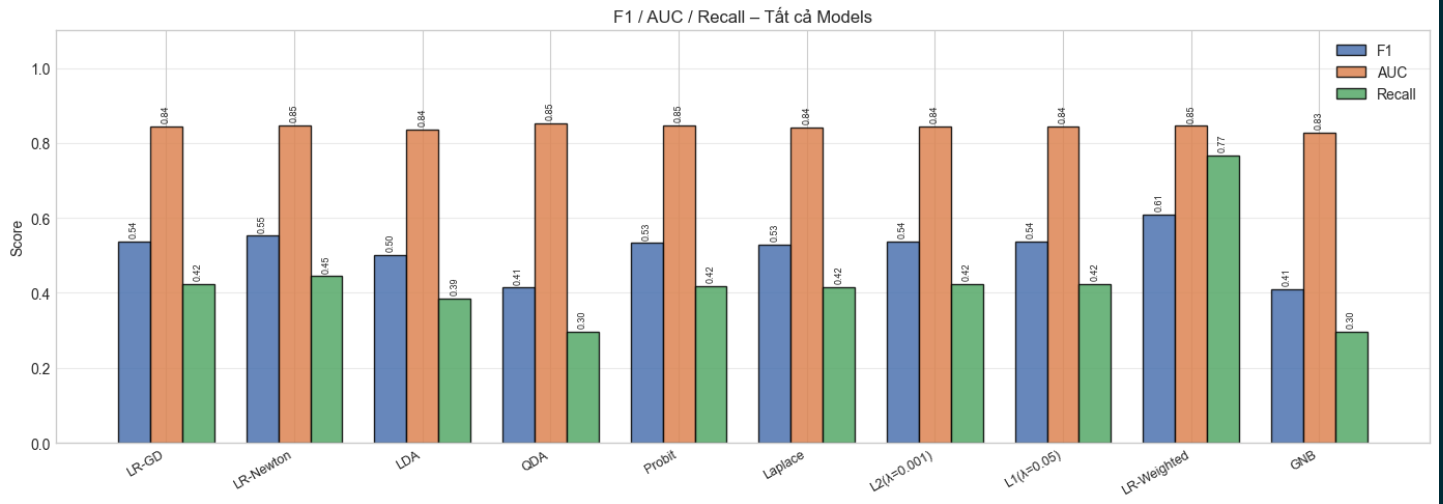
\includegraphics[width=0.9\textwidth]{figures/metrics_comparison_bar.png}
  \caption{So sánh F1, AUC, Recall trên tất cả các mô hình.}
  \label{fig:metrics_bar}
\end{figure}

\begin{figure}[H]
  \centering
  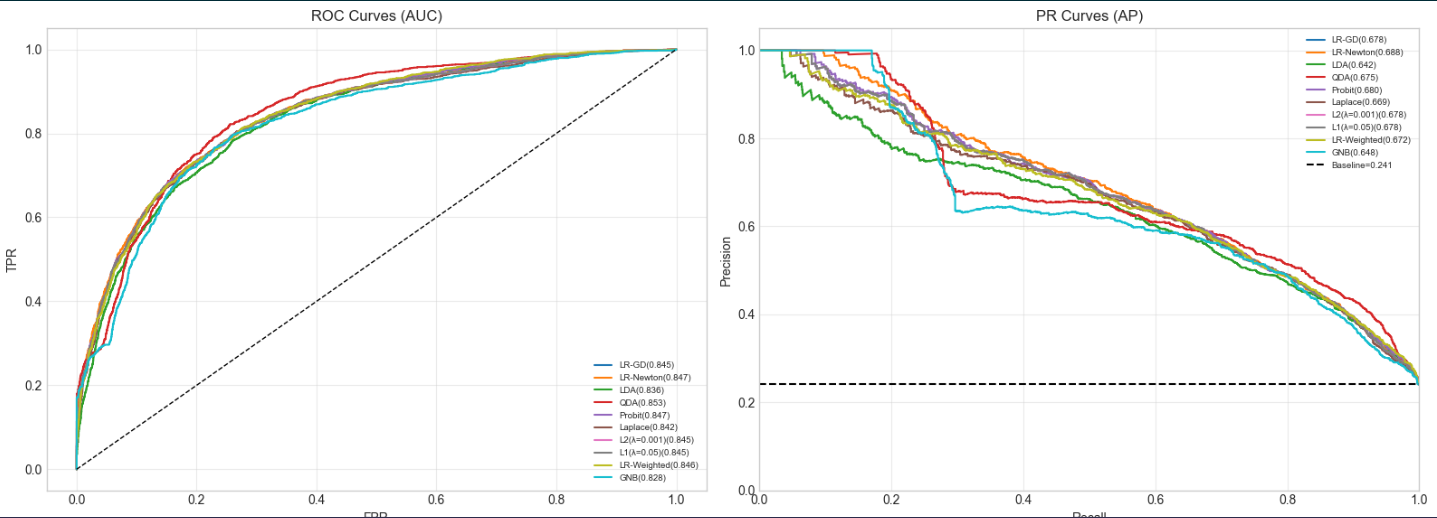
\includegraphics[width=0.9\textwidth]{figures/roc_pr_curves.png}
  \caption{ROC Curves (AUC) và Precision-Recall Curves trên tập Test.}
  \label{fig:roc_pr}
\end{figure}

\begin{figure}[H]
  \centering
  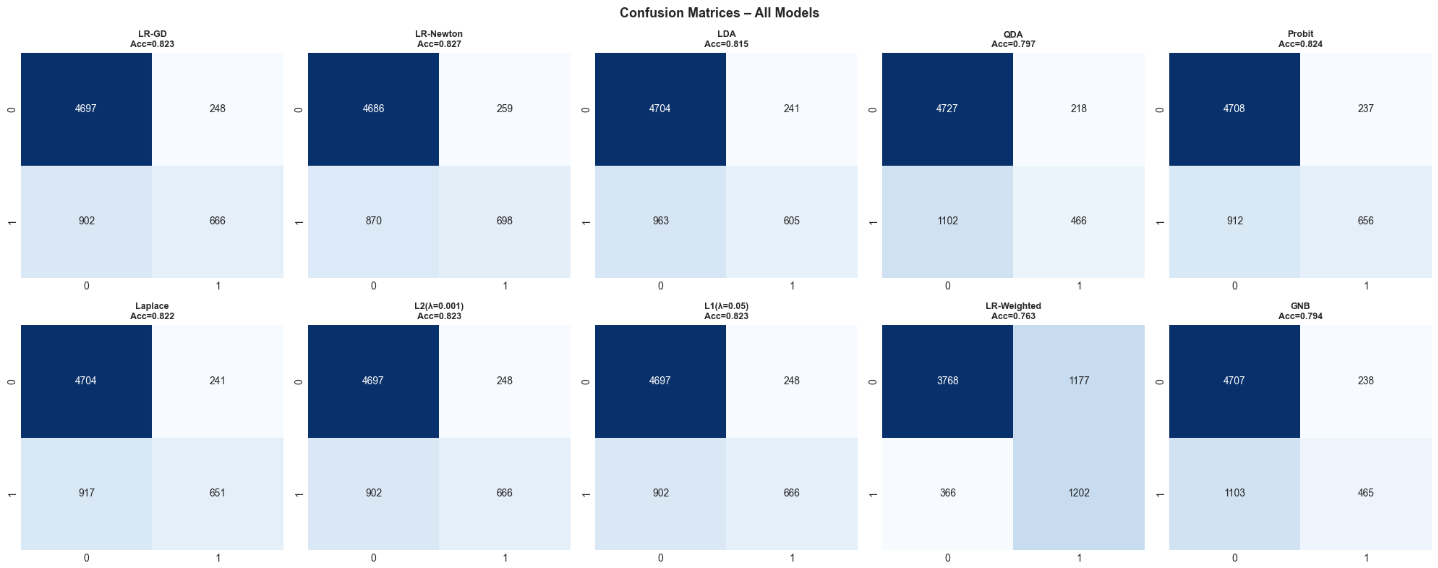
\includegraphics[width=\textwidth]{figures/confusion_matrix_grid.png}
  \caption{Grid Confusion Matrix của tất cả mô hình.}
  \label{fig:cm_grid}
\end{figure}

\subsection{Phân tích Regularization}

\begin{figure}[H]
  \centering
  \includegraphics[width=0.75\textwidth]{figures/regularization_comparison.png}
  \caption{Kết quả F1-Score theo $\lambda$ với L1 và L2 Regularization.}
  \label{fig:reg}
\end{figure}

Nhận xét:
\begin{itemize}
  \item L1 (Lasso) kích hoạt \emph{sparsity}: nhiều trọng số bằng 0 khi $\lambda$ lớn, thích hợp cho feature selection.
  \item L2 (Ridge) phân tán đều trọng số nhỏ, ít đưa về 0 hơn.
  \item Giá trị $\lambda$ tối ưu: X (L1), X (L2).
\end{itemize}

\subsection{Phân tích Calibration}

\begin{figure}[H]
  \centering
  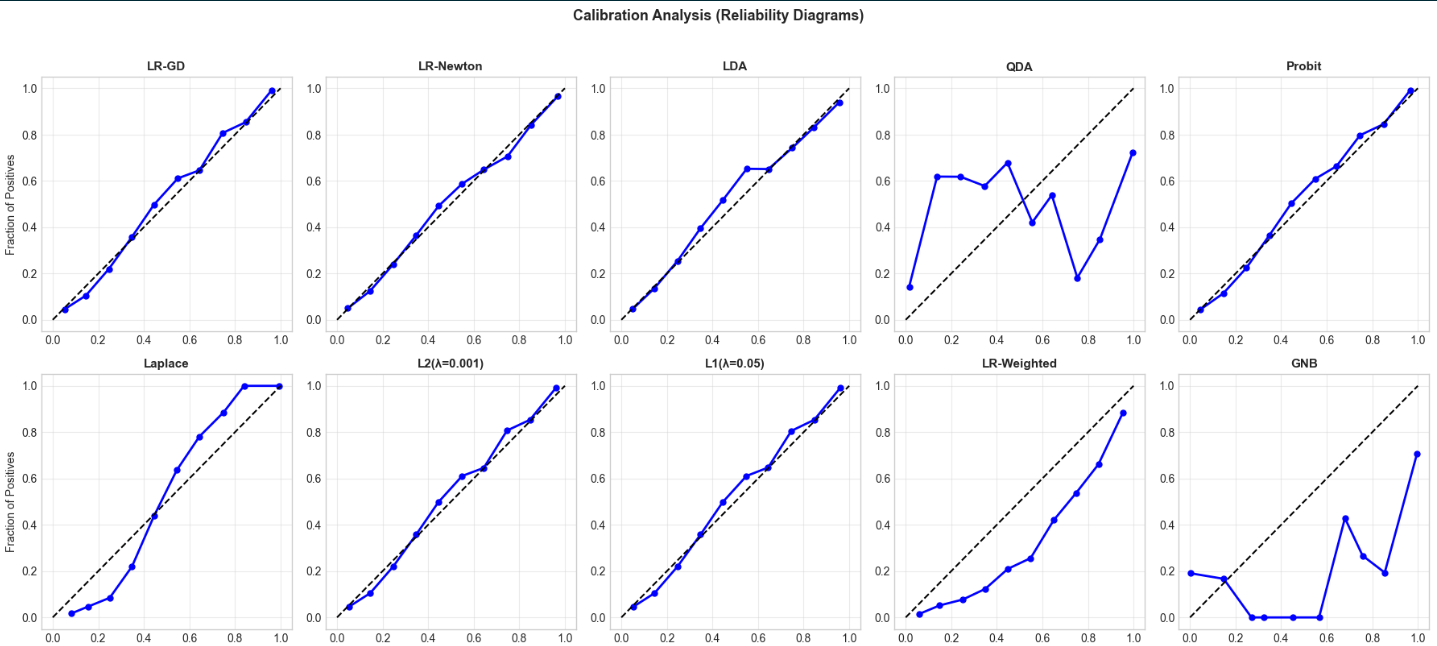
\includegraphics[width=0.9\textwidth]{figures/calibration_curves.png}
  \caption{Reliability Diagrams -- mức độ hiệu chỉnh xác suất của các mô hình.}
  \label{fig:calib}
\end{figure}

\subsection{Kiểm định thống kê (McNemar Test)}

\begin{table}[H]
  \centering
  \caption{Kết quả McNemar Test ($\alpha = 0.05$) giữa mô hình tốt nhất và các mô hình còn lại}
  \begin{tabular}{lccl}
    \toprule
    \textbf{Cặp so sánh} & $\chi^2$ & $p$-value & \textbf{Kết luận} \\
    \midrule
    Best vs. Model B & X.XX & X.XXX & Significant \\
    Best vs. Model C & X.XX & X.XXX & Not significant \\
    \ldots & & & \\
    \bottomrule
  \end{tabular}
\end{table}

Nhận xét: P-value $< 0.05$ từ chối $H_0$ (hai mô hình có hiệu năng như nhau), nghĩa là sự khác biệt có ý nghĩa thống kê.

% ============================================================
% SECTION 7 -- THẢO LUẬN
% ============================================================
\section{Thảo luận}
\label{sec:discussion}

\subsection{Mô hình tốt nhất}
% Viết nhận xét dựa trên kết quả thực nghiệm
Mô hình \textbf{[TÊN MÔ HÌNH]} đạt F1 tốt nhất ($\approx$X.XXX) và AUC $\approx$X.XXX. Nguyên nhân:
\begin{itemize}
  \item [Thêm phân tích]
\end{itemize}

\subsection{Điểm mạnh và hạn chế từng nhóm mô hình}

\begin{table}[H]
  \centering
  \caption{Ưu và nhược điểm các nhóm mô hình}
  \begin{tabular}{p{3cm}p{5cm}p{5cm}}
    \toprule
    \textbf{Mô hình} & \textbf{Ưu điểm} & \textbf{Hạn chế} \\
    \midrule
    Logistic Reg. & Đơn giản, có thể giải thích & Chỉ tuyến tính \\
    LDA & Hiệu quả nếu phân phối Gaussian & Giả định shared covariance quá mạnh \\
    QDA & Linh hoạt hơn LDA & Nhiều tham số hơn, dễ overfit \\
    Naive Bayes & Rất nhanh, ít dữ liệu & Giả định độc lập quá mạnh \\
    Kernel LR & Phi tuyến & Chậm, $O(n^2)$ \\
    Perceptron & Đơn giản & Không hội tụ nếu dữ liệu không linearly separable \\
    \bottomrule
  \end{tabular}
\end{table}

\subsection{Ảnh hưởng của imbalanced data}
Khi không dùng class weighting, các mô hình thiên về lớp đa số ($\leq$50K), dẫn đến Recall của lớp $>$50K thấp. Kỹ thuật \texttt{class\_weight='balanced'} cải thiện Recall lớp thiểu số lên $\approx$X\% nhưng có thể giảm Precision.

% ============================================================
% SECTION 8 -- KẾT LUẬN
% ============================================================
\section{Kết luận}
\label{sec:conclusion}

Báo cáo đã:
\begin{enumerate}
  \item Phân tích EDA toàn diện bộ dữ liệu Adult Census Income.
  \item Triển khai 13 mô hình phân loại \emph{from scratch} với NumPy.
  \item So sánh hiệu năng trên nhiều metric (F1, AUC, Recall, McNemar Test).
  \item Phân tích tác động của regularization và xử lý imbalanced data.
\end{enumerate}

\textbf{Kết luận chính:}
\begin{itemize}
  \item [Mô hình tốt nhất] đạt F1 $\approx$ X.XXX trên tập test.
  \item Newton-Raphson hội tụ nhanh hơn GD $\sim$\textbf{X}x về số iterations.
  \item LDA vượt QDA trên dữ liệu này vì [lý do].
  \item Class weighting cải thiện đáng kể Recall của lớp thiểu số.
\end{itemize}

% ============================================================
% PHỤ LỤC
% ============================================================
\appendix

\section{Cấu trúc code}
\label{app:code}

\begin{lstlisting}[caption={Ví dụ sử dụng LogisticRegressionGD}]
from utils import LogisticRegressionGD, plot_loss_and_cm

# Train
model = LogisticRegressionGD(
    learning_rate=0.01,
    n_iterations=1000,
    reg_lambda=0.1,
    reg_type='l2'
)
model.fit(X_train, y_train)

# Evaluate
y_pred = model.predict(X_test)
plot_loss_and_cm(model.losses, y_test, y_pred,
                 class_labels=['<=50K', '>50K'])
\end{lstlisting}

\begin{lstlisting}[caption={Ví dụ sử dụng LDA}]
from utils import LinearDiscriminantAnalysis

lda = LinearDiscriminantAnalysis()
lda.fit(X_train, y_train)
y_pred = lda.predict(X_test)

# Fisher Discriminant Ratio
fisher = lda.compute_fisher_ratios(X_train, y_train)
\end{lstlisting}

\section{Hyperparameter Tuning}
\label{app:hparam}

% Bảng tuning learning rate, lambda, ...
\begin{table}[H]
  \centering
  \caption{Grid Search Learning Rate -- Logistic Regression GD}
  \begin{tabular}{lccc}
    \toprule
    $\alpha$ & Train F1 & Val F1 & Test F1 \\
    \midrule
    0.001 & X.XX & X.XX & X.XX \\
    0.01  & X.XX & X.XX & X.XX \\
    0.1   & X.XX & X.XX & X.XX \\
    \bottomrule
  \end{tabular}
\end{table}

% ============================================================
% TÀI LIỆU THAM KHẢO
% ============================================================
\bibliographystyle{unsrt}
\begin{thebibliography}{9}

\bibitem{bishop2006}
  Christopher M. Bishop,
  \textit{Pattern Recognition and Machine Learning}.
  Springer, 2006.

\bibitem{hastie2009}
  Trevor Hastie, Robert Tibshirani, Jerome Friedman,
  \textit{The Elements of Statistical Learning}, 2nd ed.
  Springer, 2009.

\bibitem{adult_dataset}
  Ron Kohavi,
  \textit{Scaling Up the Accuracy of Naive-Bayes Classifiers: a Decision-Tree Hybrid}.
  KDD, 1996.
  UCI ML Repository: \url{https://archive.ics.uci.edu/ml/datasets/adult}.

\bibitem{goodfellow2016}
  Ian Goodfellow, Yoshua Bengio, Aaron Courville,
  \textit{Deep Learning}.
  MIT Press, 2016.

\end{thebibliography}

\end{document}
